\documentclass[12pt,a4paper]{report}
\usepackage[frenchb]{babel}
\usepackage[utf8]{inputenc}
\usepackage[export]{adjustbox}
\usepackage{verbatim}
\usepackage{amsmath}
\usepackage{amsfonts}
\usepackage{amssymb}
\usepackage{listings}
\usepackage{graphicx}
\usepackage{pgf, tikz}
	\usetikzlibrary{arrows, shapes, positioning}
\usepackage{hyperref}
\hypersetup{%
    pdfborder = {0 0 0}
}
\author{Maugey Rémy - Bernard Jérémi - De Pourquéry Benjamin - Decoudras Hadrien}
\title{Rapport projet compilation}

\usepackage{tikz}

\begin{document}

\begin{titlepage}
  \begin{sffamily}
  \begin{center}

    % Upper part of the page. The '~' is needed because \\
    % only works if a paragraph has started.
    
\includegraphics[scale=0.05]{logo.jpg}~\\[1.5cm]
    % Author and supervisor
    \begin{minipage}{0.43\textwidth}
      \begin{flushleft} \large
		MAUGEY Rémy\\
		De POURQUERY Benjamin\\
		DECOUDRAS Hadrien\\
		BERNARD Jérémi\\		
		
      \end{flushleft}
    \end{minipage}

	\topskip0pt
	\vspace*{\fill}
	\Huge{Rapport de projet technologique}\\
	\Large{Vison stéréoscopique pour robot}\\
	\vspace*{\fill}

	\vfill
    % Bottom of the page
    \begin{small}
 	Licence $3^{\text{ème}}$ année\\
 	\end{small}
    {\large \today}\\

  \end{center}
  \end{sffamily}
\end{titlepage}

\chapter{Introduction}


L'objectif de ce projet est de développer un outil implémenté sur un robot lui permettant de suivre à un mètre une personne grâce à deux caméras.\\\\

Le projet est divisé en deux parties indépendante, effectué sur les deux semestres. 
La première partie a pour but de prendre en main les outils utilisés au cours de l'année, à savoir le langage c++ (à travers qt) et la bibliothèque openCV.
Durant cette première partie sera développé un mini programme de traitement d'images. 

La deuxième partie à pour objectif de programmer le robot et d'effectuer des simulations grâce au logiciel Unity. En effet, comme le robot n'est pas forcement accessible aux membres du groupe, il est préférable de faire appelle à une simulation pour pouvoir tester les algorithmes n'importe quand.\\\\

Qt est une bibliothèque logicielle d'interface graphique, nous utiliserons cet outil pour développer l'interface du logiciel.\\

OpenCV (open computer vision) est un bibliothèque d'algorithmes de traitement d'images, de vidéos et autres. Ici elle sera utilisée pour programmer les fonctions du logiciel en rapport avec les images.\\


%Petite explication de la procédure de comment fonctionne la stereovision ...
\section{Cahier des charges}
Le cahier des charges s'oriente uniquement sur l'objectif du projet, c'est à dire sur la deuxième parties du semestre.
\subsection{Besoin fonctionnels}
	%Identifie une personne
	%Se meut
	%Calcule une distance
	Le logiciel doit prendre en entré deux images au format png représentant les images gauche et droite.
	Grâce à ces images, nous générerons la carte de disparité puis grâce à cette dernière et que caractéristique des caméras, nous pourrons générer la carte de profondeur. C'est à dire que chaque pixel de cette image correspondrons à la distance entre l'objet et les caméras.
	En fonction de cette carte de profondeur, nous serons dans la capacités de faire mouvoir le robot.
	Il sera nécessaire d'avoir une image de référence de la personne à suivre à travers une phase d'initialisation. Dans ce cas, la première image prise par le robot sera considérée comme la référence. Il faut donc que le robot soit bien placé à un mètre de la personne lors de son démarrage et que cette dernière soit la seul dans le cadre des caméras.
\subsection{Besoin non fonctionnels}
	%Robuste aux chagement de luminosité
	%changement de personne
	%chagement d'environnement
	La carte de disparité est fortement liée aux images d'entrées, de ce faite, les changements de luminosité et d'environnement peuvent poser des problèmes à cause notamment de l'utilisation d'une référence.
	Le programme doit donc être robuste à ces différents changement.\\
	Le robot doit être aussi capable de suivre la bonne personne même si une autre personne parasite rentre dans le cadre.
	
\chapter{Théorie et définitions}
%capture des images
%création de la carte de disparité + def 
%création de la carte de profondeur + def et formule
%mouvement du robot

Comme montré dans la figurer 2.1.1, le projet se structure autour d'une notion clés : Pour repérer les jambes d'une personne afin de la suivre, une carte de profondeur doit être calculée. Cette carte quand à elle est créé grâce à une carte de disparité. 

\begin{center}
\begin{tikzpicture}
	\node[draw] (capture) 	at (-4,0) 	{Images};
	\node[draw]	(disp)		at (0,0) 	{Carte de disparité};
	\node[draw] (depth)		at (5,0)	{Carte de profondeur};
	
	\draw[->]	(capture) to (disp);
	\draw[->]	(disp) to (depth);
\end{tikzpicture}\\
Figure 2.1.1 Fils rouge du projet.
\end{center}

\paragraph{Carte de disparité}
Un carte de disparité est une image où chaque pixel correspond au déplacement entre un même point dans deux images différentes. 

\begin{center}
	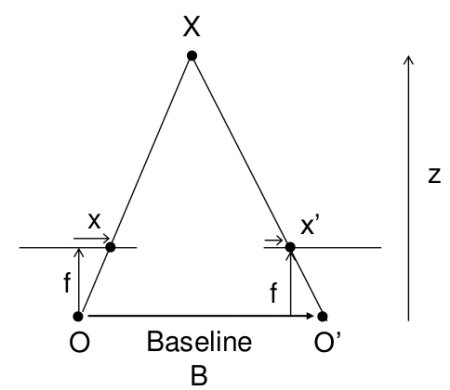
\includegraphics[scale=0.5]{disparity.jpg}\\
	Figure 2.1.2 Schéma du calcul de la carte de disparité.\footnote{Source : \url{http://docs.opencv.org/3.0-beta/doc/py_tutorials/py_calib3d/py_depthmap/py_depthmap.html}}\\
\end{center}

Comme représenté dans la figure 2.1.2, la valeur du pixel X représente le déplacement du pixel.
Les deux images sont représentées par O et O' la longueur en cm entre ces dernières par la baseline B.
\paragraph{Carte de profondeur}
La carte de profondeur est une image où chaque pixel représente la distance entre la caméra et le point dans le monde réel. Une carte de profondeur est très similaire à une carte de disparité, elle inclue cependant une référence au monde réel.\\
La formule permettant de calculer la carte de profondeur à partir de la carte de disparité résulte de l'utilisation du théorème de thalès.\\

\begin{center}
Figure 2.2.3 Formule de la carte de profondeur.\\

\begin{huge}
$\text{depth} = \frac{\frac{\text{baseline} * \text{focal}}{\frac{\text{disp}}{\text{width}} * \text{sensor size}}}{\text{référence}}$\\
\end{huge}
\end{center}
\paragraph{Légende : }
\begin{small}
\begin{enumerate}
\item[-] baseline : distance entre les deux caméras.\\
\item[-] focal : focal de l'objectif.\\
\item[-] disp : valeur du pixel de la carte de disparité.\\
\item[-] width : largeur de l'image.\\
\item[-] sensor size : taille du capteur.\\
\item[-] référence : distance voulu (dans le cadre de ce projet, en mètres donc 1000).\\
\end{enumerate}
\end{small}

On peut calculer une carte de profondeur en utilisant la formule ci-dessus sur chaque pixel ou bien utiliser une fonction d'openCV :  

\begin{lstlisting}{Language=C++}
void reprojectImageTo3D(InputArray disp, 
			OutputArray out, 
			InputArray Q, 
			bool handleMissingValues, 
			int ddepth);
\end{lstlisting}

\paragraph{Problème rencontrés}
L'utilisation de la reprojectImageTo3D implique de devoir au préalable calibrer les caméras et rectifier les images, étapes longue et non obligatoire car les caméras fournis sont suffisamment fiable. Donc nous avons opté pour la première méthode.\\

\chapter{Implémentation}

\section{Logiciel QT}
%Partie Qt
Le premier semestre c'est orienté autour du développement d'un petit programme de traitement d'image. Le programme affiche une fenêtre ainsi que plusieurs menu, l'un deux permet d'ouvrir un fichier au format png.
Le fichier doit nécessairement contenir les deux images juxtaposées pour que les algorithmes implémenté fonctionnes. On peut ensuite couper l'image en deux, on peut flouté l'image grâce à la méthode "blur" d'OpenCV. On peut aussi appliquer à l'image différent algorithme comme l'algorithme de Sobel, comme présenté sur les figures ci contre.
\begin{center}
\begin{tabular}{cc}
  \vspace{0pt} 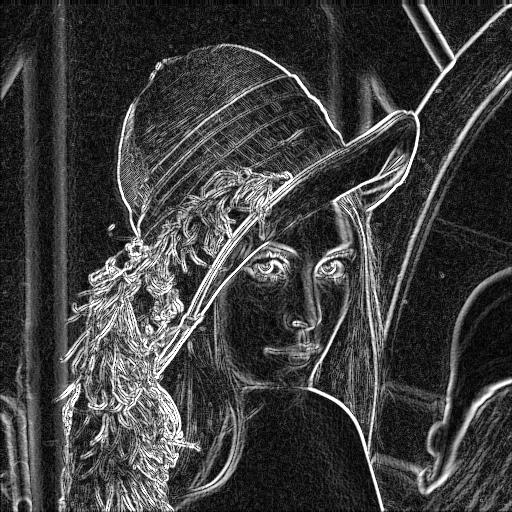
\includegraphics[width=0.49\textwidth]{sobel.jpg} &
  \vspace{0pt} 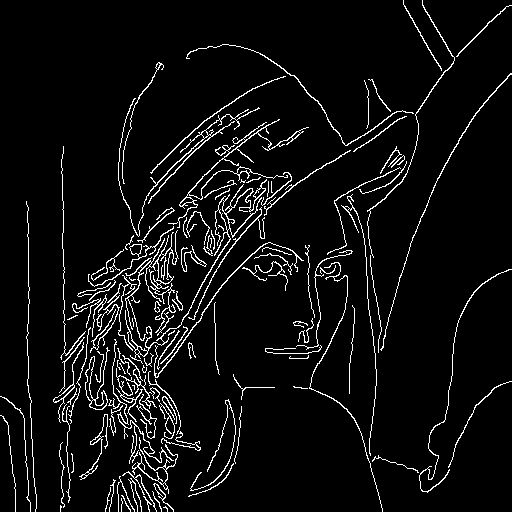
\includegraphics[width=0.49\textwidth]{canny.jpg} \\
    
  Figure 3.1.1 Sobel & Figure 3.1.2 Canny
\end{tabular}
\end{center}

Ces différentes méthodes on été implémentées dans le but de comprendre comment opencv fonctionnait, ainsi que de développer et de tester une première esquisse des fonctions que nous utiliserons dans le robot.

Il a fallu créer des méthodes de conversion d'images entre les images de qt et les images de opencv. Deux méthodes ont donc été développées,

\begin{lstlisting}{Language=C++}
cv::Mat ImageTools::imageToMat(QImage const& src);
QImage ImageTools::cvMatToImage(const cv::Mat& inMat);
\end{lstlisting}

Toutes les méthodes en rapport avec le traitement d'image ont été implémentées dans la classe \textit{imagetools}. Au début, nous conservions les images sous forme de QImage ce qui nous obligeais à convertir à chaque fois. On a fini par réécrire le programme avec des matrices opencv en images membre et la classe \textit{imagetools} sous forme d'un singleton, simplifiant le code.\\
Le logiciel permet aussi de faire de la reconnaissance de paternes grâce aux algorithmes de \textit{flann} et de surf. Cependant ce dernier n'est pas open source donc la méthode \textit{flann} est implémenté entre \textit{\#define} et n'est pas forcement proposé à l'utilisateur final.\\
Enfin, le logiciel permet de créer une carte de disparité grâce à l'algorithme \textit{stereosgbm} ou à l'algorithme \textit{stereobm}.\\

Cette partie nous à permis de prendre en main le c++ ainsi que la bibliothèque opencv. 

Grâce à ce petit outil, nous avons tester les deux algorithmes permettant de générer des cartes de disparité. Nous avons ainsi retenu \textit{stereosgbm} qui est plus performant et plus simple à utiliser. Cela nous à permis de choisir des paramètres de \textit{stereosgbm} jugés bon.\\

Le logiciel Qt prend aussi en charge diverse fonction propre à Qt et non d'OpenCV tel que le redimensionnement des images, grâce à la méthode cropImage() ou encore la possibilité de zoomer dans l'image.
\section{Simulation et test}
%partie Unity
Durant le second semestre, l'objectif était d'implémenter les algorithmes précédent pour les utiliser sur le robot. Le but est de créer une carte de profondeur grâce aux images du robot pour lui permettre de ce déplacer en fonction de la personne.\\
Comme nous n'avons forcement pas accès au robot, nous avons décidé de faire une simulation simple sur le logiciel Unity.\\

Unity est un outils qui permet dans sa fonction principale de créer des applications 3D en temps réel tel que des jeux vidéo. Il permet grâce à une interface de placer des objets dans une scènes, permet de placer une ou plusieurs caméras. Le logiciel inclus aussi une gestion avancées des interactions physique entre les objets de la scène, le tous très paramétrables grâce aux scripts. Il existe deux langages de scripts implémentés dans le logiciel, le c\# et le javascript. Durant ce projet nous avons fait le choix d'utiliser le c\#.
Ce langage de script est à la base un langage de programmation de haut niveau développé par Microsoft dans les années 2000 exclusivement pour la plateforme windows. Mais qui dans ce cas présent, est utilisé en temps que langage de scripts grâce à son implémentation libre Mono. Le c\# à une syntaxe proche du java. Mais est quand même plus souple car il prend en charge les systèmes de "namespace" ainsi que la gestion de la surcharge d'opérateurs. Le langage permet même d'utiliser des pointeurs sous forme de bloque "unsafe"\footnote{Gestion des pointeurs en c\# : \url{https://msdn.microsoft.com/en-us/library/y31yhkeb.aspx}}.

	\begin{center}
		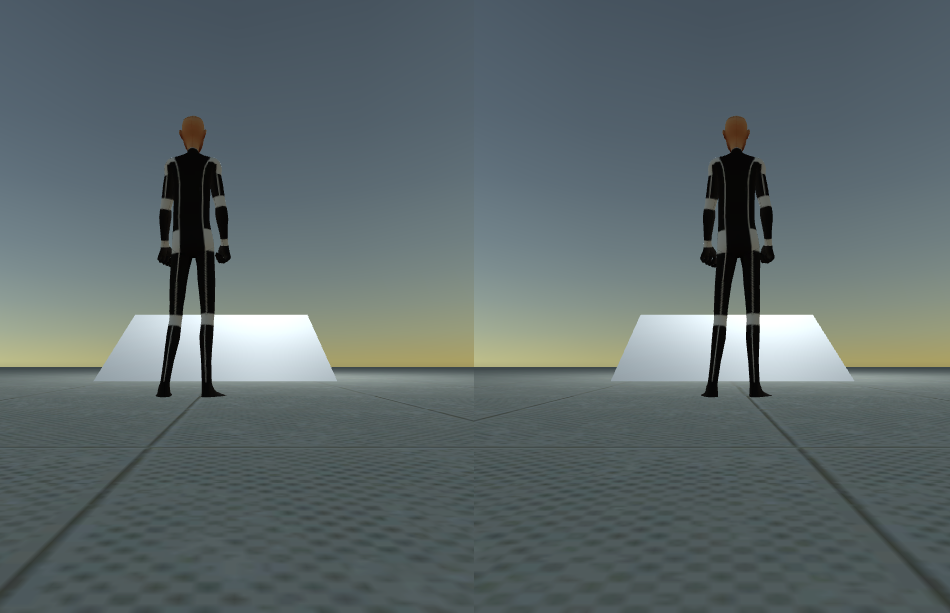
\includegraphics[scale=0.5]{Screenshot_skybox.png}
		Figure 3.2.1 Image issue de Unity\\
	\end{center}
 	
\paragraph{Problèmes rencontrés}
Le logiciel est performant pour créer des petites scènes 3d mais il est très difficilement intégrable dans git ce qui pose des problèmes pour travailler simultanément sur la simulation.

\section{Création de la bibliothèque}
Pour faire la transition entre les algorithmes, l'implémentation du robot et la simulation nous avons décidé de faire une bibliothèque externe contenant tous le code.
Cette bibliothèque a pour tâche d'être utilisée comme simple fichier objet dans le robot, relié grâce à l'édition des liens. Mais elle a aussi pour tâche d'être compilée sous forme d'une bibliothèque partagée (.so) et chargée dans Unity. Les scripts c\# d'Unity se charge juste d'appeler les fonctions c++.

Voici ci-dessous une représentation des interactions entre Unity et la bibliothèque.
\begin{center}
\begin{tikzpicture}
  	\node[draw] (camera) 	at (0, 0) 	{caméras};
  	\node[draw] (conv) 		at (0, -2) 	{Conversion vers une structure Opencv};
	\node[draw] (disp) 		at (0, -4) 	{Calcul de la carte de disparité};
	\node[draw] (depth)		at (0, -6)	{Calcul de la carte de profondeur};
  	\node[draw]	(robot)		at (0, -8)	{Gestion du mouvement du robot};

 	\draw[->] (camera) to (conv);
 	\draw[->] (conv) to (disp);
 	\draw[->] (disp) to (depth);
 	\draw[<->](depth) to (robot);
 	
 	%partie droite
	 	
	\draw (5,-2) to (5.5, -2);
	\draw (5.5,-2) to (5.5, -6);
	\draw (5,-6) to (5.5,-6);
	\draw (5.5,-4) to (6,-4);
   	\node (dll)		at (7, -4.05)	{Code c++};
   	
	\draw (5, 0) to (6, 0);
	\node (script)	at (7, 0) {Script c\#,};
	\node at (8.2, -0.5) {GetNativeTexturePtr()$^1$;};
		
	\draw[<-, dashed, draw opacity=0.5] (camera) to (-3.5, 0);
	\draw[dashed, draw opacity=0.5] (depth) to (-3.5, -6);
	\draw[black, dashed] (-3.5, -6) to[in=180, out=180] (-3.5, 0);

	\node[fill=white]	(update)	at (-5.2,-3) {update()};
	
\end{tikzpicture}

Figure 3.3.1 Interaction entre Unity et la bibliothèque.\\
\end{center}
\begin{small}
1) GetNativeTexturePtr() est une méthode c\# permettant grâce à un objet texture de récupérer sont pointeur OpengGl dans la mémoire vive.
\end{small}

\subsection{Conversion vers une structure Opencv}
La méthode GetNativeTexturePtr() renvoie un pointeur vers une image au format OpenGL (sous linux, l'image sera au format directX) dans la mémoire, c'est à dire un id OpenGL. Pour convertir cette donnée vers une matrice OpenCV, il faut dans un premier temps lié cette donnée à une texture OpenGL grâce à la fonction include dans "GL/gl.h" glBindTexture(). Ensuite il suffit de copier les données dans un tableau au au format OpenCV, c'est à dire un taille égale à la taille de la texture et une profondeur de taille 1 octet * le nombre de canaux.\\
Le standard OpenGL est de représenter l'image codée sous forme RGB et dans le sens informatique c'est à dire, le (0,0) est en haut à gauche avec les Y vers la droite et les X vers le bas. Alors que le format OpenCV est de stocker l'image sous format BGR dans le sens mathématique, c'est à dire le (0,0) en bas à droite avec les Y vers la droite et les X vers le haut.

\paragraph{Problèmes rencontrés}
Des problèmes ont été rencontrés lors de l'utilisation de la bibliothèque externe sous Unity. Ce dernier plante de temps en temps de manière obscure. (Probablement à cause de la version très précoce de Unity sous linux). Cependant malgré les nous avons décidés de continue l'intégration dans Unity tout en ayant une solution de replie.\\
Sur certaine station de travail (au Crémi), Unity ne se lancait même pas, ce qui à fortement handicapé les membres consterné (Rémy et Jérémi) et ralenti le projet.

\paragraph{Solutions envisagés}
Nous avons décidé de créer en parallèle de l'intégration à Unity un automate écrit en c++ permettant de tester les algorithmes. Un script c\# se charge de prendre une capture d'écran des deux caméras et de les écrire sur le disque. L'automate quant à lui prend en entrée les différentes images et utilise les algorithmes pour produire la carte de disparité et la carte de profondeurs.\\
L'automate est un petit programme écrit en c++ en utilisant l'outil GNU gengetopt pour gérer les argument de commande. Par exemple :\\

\begin{lstlisting}{Language=Bash}
./automate -i path/to/images -a dist
./automate -i path/to/images -a disp
\end{lstlisting}

Usage :
\begin{enumerate}
\item[] -i input "Le dossier contenant les images à traiter"
\item[] -o output "Le dossier qui contiendra les images traitées"
\item[] -p préfixe "Préfixe à appliquer aux noms de fichiers à sauvegarder"
\item[] -a action "L'action a effectuer sur chaque fichier : disp, sgbm, dist"
\end{enumerate}

\chapter{Conclusion}
%Test




\end{document}